\documentclass[11pt]{article}
\usepackage[margin=1in]{geometry}
\usepackage{amsmath,amssymb,amsthm,mathtools}
\usepackage{booktabs,tabularx,multirow}
\usepackage{graphicx}
\usepackage[hidelinks]{hyperref}
\usepackage{xcolor}
\usepackage{enumitem}
\setlist{nosep,leftmargin=*}

\newtheorem{theorem}{Theorem}
\newtheorem{proposition}[theorem]{Proposition}
\newtheorem{lemma}[theorem]{Lemma}
\newtheorem{corollary}[theorem]{Corollary}
\theoremstyle{definition}
\newtheorem{definition}[theorem]{Definition}
\theoremstyle{remark}
\newtheorem{remark}[theorem]{Remark}

\newcommand{\E}{\mathbb{E}}
\newcommand{\R}{\mathbb{R}}
\newcommand{\Var}{\mathrm{Var}}
\newcommand{\Cov}{\mathrm{Cov}}
\newcommand{\diag}{\mathrm{diag}}
\newcommand{\I}{\mathcal{I}}
\newcommand{\src}[1]{\textsf{[#1]}}

\title{Learning with Correlated Arms on the Web:\\
Certified Graph Pooling, Persistent Dynamics, and Evidence from\\ Short-Video Engagement and Wikipedia Attention}
\author{Working long version, 9 October 2026\\
\small Compiled from the \texttt{dependent\_mab} repository for later condensation into a WWW 2027 submission}
\date{}

\begin{document}
\maketitle

\begin{abstract}
Arms in web decision problems are almost never independent. Similar items share long-run appeal, and engagement shocks persist for days and spread across related items. We study bandits whose arms are correlated through two channels, written as $f_{i,t}=\mu_i+z_{i,t}$: a \emph{mean channel}, in which long-run means $\mu$ are restricted by a graph, and a \emph{fluctuation channel}, in which deviations $z$ follow a vector autoregression with graph-correlated innovations. Graphs (co-engagement, factorization, hyperlinks) are the tool for encoding correlation, not the object of study.

On the theory side we (i) reuse certified pooling results for the mean channel, including a path--clique information separation; (ii) show that certified pooling remains valid under persistent, spatially correlated, restless rewards when its confidence sets come from an exact innovation regression, and give tight scalar certificates for independent shocks (B1$'$) and, via iterated nuisance plug-in, for correlated shocks (B1$''$); (iii) show that iid certificates under-cover under bursty persistent exposure (B2); and (iv) state an innovation lower bound for dynamic regret and the principle that exploration should target uncertainty that persists.

Empirically, on KuaiRec (a nearly fully observed short-video matrix) we measure which of sixteen web graphs encode correlated appeal: collaborative and co-engagement graphs do; social, profile, location and demographic graphs barely do. Uncertified pooling has a good median but a heavy tail; certified pooling with oracle certificates halves UCB1's regret without it, while practical certificates remain too wide or invalid. Under bursty persistent exposure, iid certificates are violated in 75--90\% of runs and wrongly eliminate the best arm in 40--75\%, while innovation-regression certificates are never violated, at comparable regret. In a 100-arm AR(20) benchmark, joint predictive sampling closes 37\% of the gap between Thompson sampling and the innovation lower bound without tuning, and spatial correlation adds 15\% on top of persistence. On KuaiRec daily engagement, modelling persistence cuts regret by 38--43\% against iid Thompson sampling. On Wikipedia attention over the hyperlink graph (150 programming-language articles, four years of daily views), a drifting-level filter cuts regret 32\% and joint predictive sampling 26\% against iid Thompson sampling; shocks are strongly correlated but through a domain-wide factor, so hyperlinks add nothing beyond it.
\end{abstract}

\tableofcontents
\newpage

%=====================================================================
\section{Introduction}
%=====================================================================

Recommendation slots, trending modules, headline tests and promotion widgets are bandit problems whose arms are correlated. Two kinds of correlation recur on the web.
\begin{itemize}
\item \textbf{Correlated long-run appeal.} Videos watched by the same people are liked by the same people; articles linked to each other attract related readers. A learner that knows this can reject groups of arms without sampling each one.
\item \textbf{Correlated persistent fluctuations.} Engagement with an item drifts for days; a news event lifts a cluster of related pages at once. Observations are then neither independent over time nor across arms.
\end{itemize}
Platforms already hold graphs that encode such structure: social networks, co-engagement logs, embeddings, hyperlinks. Graph bandits (spectral, clustered, Laplacian-regularized) take one such graph and assume rewards are smooth on it. Two questions are left open, and both are specific to the web.
\begin{enumerate}
\item \emph{Which correlation can a learner trust?} Web graphs are by-products, not designed priors. Uncertified smoothing on a misaligned graph incurs linear regret.
\item \emph{How much is each observation worth when rewards persist?} Persistence makes each observation less informative about long-run means (the long-run variance) and more informative about near-term rewards. Methods built for iid rewards produce invalid confidence statements under persistence, especially when exposure is bursty, as it is in daily slates and batched updates.
\end{enumerate}

\paragraph{Model and message.} We write every reward as $f_{i,t}=\mu_i+z_{i,t}$. The mean channel restricts $\mu$ by a graph certificate; the fluctuation channel lets $z$ follow an autoregression whose innovations are correlated through a graph. iid bandits are the special case with no persistence and diagonal innovations; static graph bandits add only the mean channel. Our message is that correlation is valuable but dangerous: graphs let learners pool, but only certified pooling is safe; persistence must enter the confidence sets, or certificates fail; and exploration must target uncertainty that will persist.

\paragraph{Contributions.}
\begin{enumerate}
\item A two-channel model of correlated arms with two regret notions (mean regret against the best long-run mean; dynamic regret against the full-current-state oracle), unifying static graph bandits and restless autoregressive bandits (Section~\ref{sec:model}).
\item Mean-channel theory reused from companion work \src{A}: certified pooling (SP-UCB) regret, the path--clique information separation, graph-error inflation, and the misalignment counterexample (Section~\ref{sec:mean}).
\item \textbf{Bridging results (new).} Certified pooling built on the innovation regression of \src{S} is valid under persistent, correlated, restless sampling (B1), with a regret bound in realized information; tight scalar certificates for independent shocks (B1$'$) and for correlated shocks via iterated nuisance plug-in (B1$''$); failure of iid certificates under persistence (B2); and long-run substitution of the mean-channel constants with a slate contrast gain (B3) (Section~\ref{sec:bridge}).
\item Fluctuation-channel results: an innovation lower bound for dynamic regret, exact contrast information, joint-filter policies, and the exploration-targeting principle supported by both simulation and real data (Section~\ref{sec:fluct}).
\item Evidence on two real web platforms and a controlled benchmark: KuaiRec (graph alignment for sixteen graphs, item and user pooling, daily engagement dynamics), a 100-arm AR(20) spatiotemporal benchmark with coverage tests, and Wikipedia attention over the hyperlink graph (Section~\ref{sec:exp}).
\end{enumerate}

\paragraph{Provenance labels.} Results proved in companion manuscripts in the same repository are labelled \src{A} (\texttt{research/alignment\_paper}), \src{S} (\texttt{research/spatiotemporal\_bandits}), \src{P} (\texttt{research/predictive\_ar1}, \texttt{two\_arm\_ar1}, \texttt{ar\_p\_bandits}) and \src{N} (\texttt{research/graph\_spectral\_bandits.md}). Results first stated here are labelled \src{New}.

%=====================================================================
\section{Related work}
%=====================================================================

\paragraph{Graph and structured bandits.} Spectral bandits treat arms as graph nodes with smooth means and achieve regret governed by an effective dimension (Valko et al., ICML 2014; Koc\'ak et al., JMLR 2020). GRUB studies best-arm identification with graph side information (Thaker et al., NeurIPS 2022). Clustered bandits share observations within known clusters (Pandey et al., ICML 2007; Clus-UCB; hierarchical Thompson sampling, Hong et al., ICML 2022). Structured bandits with instance-optimal exploration are covered by OSSB (Combes et al., NeurIPS 2017); unimodal and Lipschitz structures by OSUB and zooming algorithms. Multi-user graph bandits pool across users through a social graph (GOB.Lin, Cesa-Bianchi et al., NeurIPS 2013), learned clusters (CLUB, Gentile et al., ICML 2014; LOCB, Ban and He, WWW 2021), graph neural networks (Qi et al., KDD 2023), or a Laplacian-fused kernel (Wu and Amini, ICLR 2026). Robustness to noisy graphs is studied for spectral projection (Mondal et al., 2026) and clustering with misspecified user models (Wang et al., NeurIPS 2023). The selection-index line (Sun, Li and Fu, WSC 2019; Zhou, Fu and Ryzhov, Operations Research 2024) studies final selection with graph smoothing; our mean channel continues it for cumulative regret.

\paragraph{Temporally dependent and restless bandits.} Time-varying Gaussian-process bandits model a spatial GP evolving by a Markov recurrence (Bogunovic et al., AISTATS 2016) and show a linear-regret obstruction at fixed variation. Restless bandits driven by linear Gaussian dynamics use joint Kalman filtering across arms (Gornet and Sinopoli, L4DC 2024). Latent autoregressive bandits learn shared AR drivers (Trella et al., RLC 2025); AR-dependent non-stationary bandits are studied by Chen et al. (NeurIPS 2023). Predictive Sampling explores only information that remains useful (Liu, Van Roy and Xu, AISTATS 2023). Candidate-prior elimination handles unknown time-varying priors (Ziomek et al., AISTATS 2025).

\paragraph{Positioning.} Joint filtering, time-varying GP-UCB, knowledge gradient, Predictive Sampling and spectral regularization are established tools, credited as such. Our contributions are the two-channel framing for web arms, the certified-pooling bridge under persistence (B1--B3), and measurements of which web graphs encode which kind of correlation.

%=====================================================================
\section{Model}\label{sec:model}
%=====================================================================

There are $N$ arms. In round $t$ the learner pulls one arm $a_t$ (or a slate $S_t$ of $k$ arms) and observes
\begin{equation}
Y_t=\mu_{a_t}+z_{a_t,t}+\xi_t,\qquad z_t=\sum_{r=1}^{p}A_r z_{t-r}+\eta_t,\qquad \eta_t\sim N(0,Q_G),\qquad \xi_t\sim N(0,r).
\end{equation}
Every arm evolves every round (restless); only pulled arms are observed. The $A_r$ are stable; $Q_G$ is an innovation covariance built from a graph.

\paragraph{Mean channel.} The long-run means $\mu\in[0,1]^N$ are fixed and unknown. A graph supplies either a partition $\{C_1,\dots,C_M\}$ with certified diameters $\varepsilon_c\ge\max_{i\in C_c}\mu_i-\min_{i\in C_c}\mu_i$, or an energy certificate $\mu_c^\top L_c\mu_c\le S_c^2$ on each component, which yields diameters through effective resistance (Lemma~\ref{lem:resistance}).

\paragraph{Regret.} Mean regret is $\mathcal R_T=\sum_t(\mu^\star-\mu_{a_t})$. Dynamic regret is $\sum_t(\max_i f_{i,t}-f_{a_t,t})$, against the oracle that sees every current reward. With slates, both are summed over the slate against the oracle's top $k$.

\paragraph{Special cases.} iid stochastic bandits: $A_r=0$, $Q_G$ diagonal, no certificate. Static graph bandits: $A_r=0$ with a mean certificate. Restless AR bandits: no mean certificate.

\paragraph{What graphs encode.} A graph can enter through the mean channel (pooling long-run estimates), the fluctuation channel (shrinking the innovation covariance toward a graph kernel), or both. Section~\ref{sec:exp} measures empirically which web graphs carry which channel.

%=====================================================================
\section{Mean channel: certified pooling}\label{sec:mean}
%=====================================================================

This section restates results from \src{A} and \src{N} in the present notation; proofs are in \src{A}.

\begin{lemma}[Energy certifies reward diameter \src{A}]\label{lem:resistance}
If $\mu_c^\top L_c\mu_c\le S_c^2$ on a connected component, then $|\mu_i-\mu_j|\le S_c\sqrt{r^{\rm eff}_{ij}}$, so $\varepsilon_c=\min\{1,S_c\sqrt{D^{\rm eff}_c}\}$ is a valid diameter, where $D^{\rm eff}_c$ is the resistance diameter.
\end{lemma}

\paragraph{SP-UCB \src{A}.} With $b(n)=\sigma\sqrt{2\ell/n}$, $\ell=\log(2(K+M)T/\delta)$, arm upper bounds $u_i=\bar Y_i+b(n_i)$ and pooled component means $\hat p_c$ over $N_c$ pulls, SP-UCB selects the component maximizing
\begin{equation}
U_c=\min\{\max_{i\in C_c}u_i,\ \hat p_c+b(N_c)+\varepsilon_c\}
\end{equation}
and pulls its best arm.

\begin{theorem}[Alignment-sensitive regret \src{A}]\label{thm:spucb}
With valid certificates, on an event of probability at least $1-\delta$,
\[
\mathcal R_T\le\sum_{c\in\mathcal O}A_c+\sum_{c\notin\mathcal O}\min\{A_c,H_c\},\quad
A_c=\sum_{i\in C_c:\Delta_i>0}\Big(\Delta_i+\frac{8\sigma^2\ell}{\Delta_i}\Big),\quad
H_c=(\Gamma_c+\varepsilon_c)\Big(1+\frac{8\sigma^2\ell}{(\Gamma_c-\varepsilon_c)^2}\Big)
\]
for $\varepsilon_c<\Gamma_c$ (and $H_c=\infty$ otherwise), where $\Gamma_c$ is the gap between the best arm and component $c$'s best arm and $\mathcal O$ are the optimal components.
\end{theorem}

\paragraph{Geometry, not diameter \src{A}.} A normalized path and a normalized clique on $m$ arms can share means, energy budget and resistance diameter, yet their information costs differ by a factor growing with $m$: endpoint observations reject a path component, while a clique requires arm-wise exploration. A graph-design elimination policy (GDE-UCB) attains the path's improved arm-count dependence. The first-order cost of loosening a certificate is governed by the resistance radius $\rho_L$, the smallest enclosing ball in the resistance embedding.

\paragraph{Estimated graphs \src{A}.} If $(1-\eta)L\preceq\hat L\preceq(1+\eta)L$ on the constant-free subspace, inflating a valid energy radius to $\sqrt{1+\eta}\,S$ yields a valid certificate for $\hat L$.

\paragraph{Misalignment \src{N}.} For $\mu=(1,0.9,0)$ with only arms 1 and 3 connected and $\lambda=1$, the smoothed means $(I+\lambda L)^{-1}\mu=(2/3,0.9,1/3)$ have a different maximizer; a fixed smoothed index with an ordinary bonus incurs $0.1T+O(\log T)$ regret. Uncertified smoothing can therefore be linearly worse than ignoring the graph.

%=====================================================================
\section{Bridge: certified pooling under persistent, correlated rewards}\label{sec:bridge}
%=====================================================================

\subsection{The innovation regression \src{S}}

Condition on a candidate mean $\mu$. Because $z$ is independent of $\mu$, the lag state satisfies $s_t\mid\mu,\mathcal H_t\sim N(g_t+D_t\mu,P_t)$ with $g_t,D_t,P_t$ computed by a Kalman recursion that does not depend on $\mu$.

\begin{theorem}[Predictable innovation experiments \src{S}]\label{thm:innov}
For the chosen arm, with $v_t=e_{a_t}+D_t^\top\ell_{a_t}$, $d_t=\ell_{a_t}^\top P_t\ell_{a_t}+r$ and $u_t=v_t/\sqrt{d_t}$,
\[
R_t=\frac{Y_t-\ell_{a_t}^\top g_t}{\sqrt{d_t}}=u_t^\top\mu+\epsilon_t,\qquad \epsilon_t\mid\mathcal H_t\sim N(0,1),
\]
with $u_t$ predictable. The information $\I_T=\sum_{t\le T}u_tu_t^\top$ and score $q_T=\sum u_tR_t$ agree with the dense likelihood for each recorded path.
\end{theorem}

\begin{theorem}[All-time confidence \src{S}]\label{thm:alltime}
With $J_T=H+\I_T$, $H=\alpha I+\lambda L$, $\hat\mu_T=J_T^{-1}q_T$ and
$\beta_T=\sqrt{\log(\det J_T/\det H)+2\log(1/\delta)}+\sqrt{\alpha B^2+\lambda S^2}$, with probability at least $1-\delta$, for all $T$ and all $v$,
$|v^\top(\hat\mu_T-\mu)|\le\beta_T\|v\|_{J_T^{-1}}$.
\end{theorem}

\subsection{B1: validity and regret}

\paragraph{SP-UCB-ST.} Define $U_i=\hat\mu_i+\beta_t\|e_i\|_{J_t^{-1}}$ and
\[
U_c=\min\Big\{\max_{i\in C_c}U_i,\ \min_{w\in\Delta(C_c)}\big(w^\top\hat\mu+\beta_t\|w\|_{J_t^{-1}}\big)+\varepsilon_c\Big\}.
\]

\begin{theorem}[B1 \src{New}]\label{thm:b1}
With valid certificates and correctly specified dynamics:
\begin{enumerate}
\item With probability at least $1-\delta$, at every round, $U_i\ge\mu_i$ for all arms and $U_c\ge v_c=\max_{i\in C_c}\mu_i$ for all components.
\item If each pull in $C_c$ raises $1/\min_{w\in\Delta(C_c)}\|w\|^2_{J_t^{-1}}$ by at least $\iota_c$ and each pull of arm $i$ raises $1/\|e_i\|^2_{J_t^{-1}}$ by at least $\iota_i$, then on the same event $N_c(T)\le1+4\beta_T^2/(\iota_c(\Gamma_c-\varepsilon_c)^2)$ and $n_i(T)\le1+4\beta_T^2/(\iota_i\Delta_i^2)$; Theorem~\ref{thm:spucb} holds with $8\sigma^2\ell$ replaced by $4\beta_T^2/\iota$.
\item For independent AR(1) arms with $0\le\varphi<1$, $\iota_i\ge(1-\varphi)^2/(V+r)$ and $\iota_c\ge|C_c|(1-\varphi)^2/(V+r)$.
\end{enumerate}
\end{theorem}
\begin{proof}
(1) Theorem~\ref{thm:alltime} holds for all contrasts simultaneously, hence for every $e_i$ and every $w$ in every simplex. For $w\in\Delta(C_c)$, $w^\top\mu\ge v_c-\varepsilon_c$, so both terms of $U_c$ bound $v_c$. Minimizing over $w$ is free because the event does not depend on $w$.
(2) If $c$ is selected, $\mu^\star\le U_c\le v_c+\varepsilon_c+2\beta_t\|w\|_{J_t^{-1}}$ for the minimizing $w$, so $\min_w\|w\|^2_{J_t^{-1}}\ge(\Gamma_c-\varepsilon_c)^2/(4\beta_t^2)$, while information growth makes it at most $1/(\iota_c(N_c-1))$. Arms are identical. Summation follows Theorem~\ref{thm:spucb}.
(3) With independent arms the information is diagonal. The coefficient of $\mu_i$ in a pull of arm $i$ is $1-\varphi^h s$, where $h\ge1$ is the gap since the last observation and $s\in[0,1]$ is the filter's estimate after unit residuals (each filter step is a convex combination of $\varphi$ times the previous estimate and the new residual). Hence the coefficient is at least $1-\varphi$, and $d\le V+r$. For a component, take $w$ proportional to the diagonal information.
\end{proof}

\begin{remark}[Why B1 is too wide]
$\beta_T$ carries the $N$-dimensional log-determinant, about $\sqrt{N\log T}$. With 20 arms and $T=20{,}000$ it is about 12 standard errors, against about 5.5 for a per-arm bound; empirically B1 eliminated no arm in 20,000 rounds (Section~\ref{sec:exp-cert}).
\end{remark}

\subsection{B1$'$: tight certificates for independent shocks}

\begin{proposition}[B1$'$ \src{New}]\label{prop:b1p}
Let $Q_G$ be diagonal and $H=\alpha I$. Then every $u_t$ has a single nonzero entry, $\I_t$ is diagonal and each arm's score $W_i=\sum_{t:a_t=i}u_t\epsilon_t$ is a scalar martingale. With $\delta'=\delta/(N+M)$, $J_c=\alpha+\sum_{i\in C_c}\I_{ii}$ and $q_c=\sum_{i\in C_c}q_i$,
\[
U_i=\frac{q_i}{J_{ii}}+\frac{\sqrt{2\log(\sqrt{J_{ii}/\alpha}/\delta')}+\sqrt\alpha}{\sqrt{J_{ii}}},\qquad
U^{\rm pool}_c=\frac{q_c}{J_c}+\frac{\sqrt{2\log(\sqrt{J_c/\alpha}/\delta')}+\sqrt\alpha}{\sqrt{J_c}}+\varepsilon_c
\]
satisfy $U_i\ge\mu_i$ and $U_c^{\rm pool}\ge v_c$ at every round with probability at least $1-\delta$.
\end{proposition}
\begin{proof}
Each $(q_i,J_{ii})$ is the scalar case of Theorem~\ref{thm:alltime}; the one-dimensional method of mixtures applies and the regularization bias is at most $\sqrt\alpha$. The pooled statistic estimates the information-weighted average of the pulled arms' means, which is at least $v_c-\varepsilon_c$; its error is a scalar martingale with quadratic variation $J_c-\alpha$. A union bound over the $N+M$ scalar processes completes the proof.
\end{proof}

\subsection{B1$''$: correlated shocks by iterated nuisance plug-in}

With correlated shocks, $u_t$ couples arms: observing one arm subtracts predicted shared noise, which involves other arms' means. Write $G=J-\alpha I$ (realized information). For arm $i$,
\[
q_i-\sum_{j\ne i}G_{ij}m_j=G_{ii}\mu_i+\sum_{j\ne i}G_{ij}(\mu_j-m_j)+W_i,
\]
where $W_i=\sum_t u_{t,i}\epsilon_t$ is a scalar martingale with quadratic variation $G_{ii}$ and $m_j$ is any plug-in value.

\begin{proposition}[B1$''$ \src{New}]\label{prop:b1pp}
Let $E$ be the event that every scalar mixture bound $|W_i|\le\sqrt{2J_{ii}\log(\sqrt{J_{ii}/\alpha}/\delta')}$ (and its component analogue below) holds for all rounds; $\Pr(E)\ge1-\delta$. On $E$, the map that sends intervals $[l_j,h_j]\ni\mu_j$ to
\[
\hat\mu_i\pm\rho_i,\qquad \hat\mu_i=\frac{q_i-\sum_{j\ne i}G_{ij}m_j}{J_{ii}},\qquad
\rho_i=\frac{\sqrt{2J_{ii}\log(\sqrt{J_{ii}/\alpha}/\delta')}+\alpha+\sum_{j\ne i}|G_{ij}|h_j}{J_{ii}},
\]
with $m_j$ and $h_j$ the midpoint and half-width of $[l_j,h_j]$, maps true-containing intervals to true-containing intervals. Iterating from $[0,1]$ therefore yields valid intervals. For components, write $\mu_i=\theta_c+d_i$ with $\theta_c$ the component midrange and $|d_i|\le\varepsilon_c/2$; applying the same argument to $\theta$ with design $P^\top u_t$ ($P$ the membership matrix) gives a valid pooled bound $\hat\theta_c+\rho_c+\varepsilon_c/2\ge v_c$, where $\rho_c$ includes the deterministic deviation term $\sum_i|(P^\top G)_{ci}|\varepsilon_{c(i)}/2$.
\end{proposition}
\begin{proof}
On $E$, the error of $\hat\mu_i$ is $[\,{-\alpha\mu_i}+\sum_{j\ne i}G_{ij}(\mu_j-m_j)+W_i]/J_{ii}$, bounded by $\rho_i$ whenever each $\mu_j$ lies in its interval. Induction over iterations keeps every interval true-containing. For components, $\sum_t(P^\top u_t)_c\sum_iu_{t,i}d_i=\sum_i(P^\top G)_{ci}d_i$, which is deterministic given the data and bounded by the stated term.
\end{proof}

\begin{remark}
With independent shocks, $G$ is diagonal, the cross terms vanish and the component deviation term equals $\varepsilon_c/2$ times the information, so the pooled bound reduces to SP-UCB's $\hat p_c+b(N_c)+\varepsilon_c$ structure. B1$''$ thus generalizes both SP-UCB and B1$'$.
\end{remark}

\subsection{B2: iid certificates fail under persistence}

\begin{proposition}[B2 \src{New}]\label{prop:b2}
For one arm sampled on $n$ consecutive rounds with stationary AR(1) persistence $\varphi\in(0,1)$, $r=0$ and $\Var(z)=V$,
\[
\Var(\bar Y_n)=\frac Vn\Big[\frac{1+\varphi}{1-\varphi}-\frac{2\varphi(1-\varphi^n)}{n(1-\varphi)^2}\Big],
\]
so the iid radius $\sqrt{2V\ell/n}$ has miscoverage tending to $2\Phi(-\sqrt{2\ell(1-\varphi)/(1+\varphi)})$, which tends to 1 as $\varphi\to1$ at fixed $\ell$.
\end{proposition}
\begin{proof}
Sum the autocovariances $V\varphi^{|s-u|}$; the sample mean is Gaussian.
\end{proof}

The failure needs consecutive or bursty exposure. With one-at-a-time interleaved sampling, repeat pulls of an arm are far apart and the inflation is much smaller (Section~\ref{sec:exp-cert}).

\subsection{B3: long-run substitution and the slate contrast gain}

\begin{proposition}[B3 \src{New}, combining \src{A} and \src{S}]\label{prop:b3}
(1) Under long consecutive runs or full fields with common AR coefficients, per-observation mean information converges to $c^2Q_G^{-1}$ with $c=1-\sum_ra_r$ \src{S}; the constants of Theorem~\ref{thm:spucb}, the path--clique separation and the information-design lower bound of \src{A} then hold with $\sigma^2$ replaced by the long-run variance $q/c^2$ (for AR(1), $V(1+\varphi)/(1-\varphi)$). (2) When a slate of $k$ arms is observed in one round, two arms with innovation correlation $\rho$ have long-run contrast variance $2q(1-\rho)/c^2$ per round, so positively correlated shocks make comparisons, and therefore component rejection, cheaper by the factor $1-\rho$.
\end{proposition}

Part (1) is the consecutive-run limit; for single pulls at gaps the information is schedule-dependent \src{S,P}. Part (2) is a direct Gaussian calculation.

%=====================================================================
\section{Fluctuation channel}\label{sec:fluct}
%=====================================================================

\paragraph{Joint filter.} Stack $(\mu,z_t,\dots,z_{t-p+1})$; a single Gaussian belief is updated by each observation and propagated through the companion dynamics. One observation updates every arm and every lag \src{S}. We verify the implementation against dense Gaussian conditioning over the full node-time covariance.

\begin{proposition}[Innovation lower bound \src{S,P}]\label{prop:floor}
With $\mathcal G(\mu,K)=\E\max_i(\mu_i+Z_i)$, $Z\sim N(0,K)$, stationary covariance $K_0$ and innovation covariance $Q_G$, every causal policy has dynamic regret at least $T\{\mathcal G(\mu,K_0)-\mathcal G(\mu,K_0-Q_G)\}$.
\end{proposition}

\paragraph{Contrast information \src{S}.} Observing arm $a$ reduces the variance of a future difference $f_{j,t+s}-f_{k,t+s}$ by $(C_{j,s;a}-C_{k,s;a})^2/d_a$. A shock common to $j$ and $k$ cancels: correlated shocks help comparisons and dilute ranking information about transient states.

\paragraph{Policies.} On the joint belief we compare: greedy (largest predictive mean); current-state Thompson sampling (a joint draw of current rewards); UCB on the current state with bonus $m$ predictive standard deviations; the exact two-period score $Q_a=m_a+\E_Z\max_j(\ell_j+u^{(a)}_jZ)$ \src{S,P}; and joint predictive sampling, which samples only the part of current uncertainty that next round's rewards would reveal, $B=CV^{-1}C^\top$ with $C=\Cov(f_t,f_{t+1})$ and $V=\Var(f_{t+1})$ (a one-step specialization of Predictive Sampling). A persistent-sampling variant samples only the long-run means and sets the fluctuation to its conditional mean.

\paragraph{Exploration targeting.} Current-state Thompson sampling samples the fresh innovation, which carries no information that persists; exploring it is pure cost. Predictive and persistent sampling avoid this. Whether exploration pays at all depends on how many observations each arm will receive, which the experiments make concrete.

%=====================================================================
\section{Experiments}\label{sec:exp}
%=====================================================================

All code is in \texttt{experiments/}; every number below is produced from saved result files. Section~\ref{sec:repro} lists commands.

\subsection{KuaiRec data and sixteen web graphs}

KuaiRec 2.0 contains a small matrix of 1,411 users $\times$ 3,327 videos that is 99.6\% observed (17,827 blocked pairs) and a big matrix of 7,176 users $\times$ 10,728 videos (12.53M interactions, 16.3\% dense). The evaluation users and videos are subsets of the big matrix, and the big matrix contains \emph{no} evaluation (user, video) pair. Graphs are therefore leakage-free by construction: user-side signals use only non-evaluation videos and video-side signals only non-evaluation users. The social network covers 146 of the 1,411 evaluation users with 47 edges (80 users have a friend in the evaluation set), so the social graph is reported but cannot carry results. Rewards use $\min(\text{watch ratio},5)/5$ (R1); the median watch ratio is 0.77 and 4.6\% exceed 2.

Graphs are union-$k$NN ($k\in\{5,10,20\}$), with Laplacians scaled to mean degree one so that a random graph has smoothness quotient $\mu^\top L\mu/\|\mu-\bar\mu\|^2\approx1$. Each real graph is compared with a degree-preserving rewiring and an Erd\H{o}s--R\'enyi graph. Table~\ref{tab:graphs} defines them.

\begin{table}[t]\centering\small
\begin{tabularx}{\linewidth}{lX}
\toprule
Graph & Construction \\
\midrule
U-coeng & Jaccard on sets of fully watched non-evaluation videos (watch ratio $\ge1$) \\
U-coeng-idf / U-coauthor & Cosine on IDF-weighted engagement; by video, or aggregated by author \\
U-mf / I-mf & PureSVD factors (rank 64) on leakage-free splits \\
U-cotag / U-cotime & Per-tag taste profile; hour-of-day activity profile \\
U-soc & Friend lists \\
U-feat / U-geo / U-demo & Profile fields; same city (1) or province (0.3); gender, age, phone brand, price band \\
I-coeng / I-coauthor & IDF-weighted engagement from non-evaluation users; same author \\
I-tag / I-cat & Jaccard on tags; three-level category tree \\
\bottomrule
\end{tabularx}
\caption{The sixteen KuaiRec graphs.}\label{tab:graphs}
\end{table}

\subsection{Which graphs encode correlated appeal}

\begin{table}[t]\centering\small
\resizebox{\linewidth}{!}{%
\begin{tabular}{lcrccc}
\toprule
Graph & Side & Edges & Quotient (real / rewired) & Personal-taste corr. (real / random) & Choice cost $\lambda{=}10$ (real / rewired) \\
\midrule
I-mf & I2I & 25,492 & 0.756 / 0.961 & 0.046 / 0.002 & 0.117 / 0.019 \\
I-coauthor & I2I & 30,080 & 0.805 / 1.006 & 0.004 / 0.002 & 0.040 / 0.184 \\
I-cat & I2I & 29,558 & 0.908 / 0.985 & 0.010 / 0.002 & 0.099 / 0.079 \\
I-tag & I2I & 30,094 & 0.943 / 1.010 & 0.010 / 0.002 & 0.100 / 0.054 \\
I-coeng & I2I & 31,680 & 1.098 / 1.302 & 0.034 / 0.002 & 0.131 / 0.037 \\
U-coeng & U2U & 12,563 & 0.649 / 0.791 & 0.020 / 0.000 & 0.284 / 0.291 \\
U-coeng-idf & U2U & 11,193 & 0.748 / 0.860 & 0.018 / 0.001 & 0.294 / 0.296 \\
U-coauthor & U2U & 11,182 & 0.761 / 0.871 & 0.018 / 0.000 & 0.296 / 0.294 \\
U-cotag & U2U & 10,716 & 0.842 / 0.884 & 0.004 / 0.001 & 0.299 / 0.297 \\
U-mf & U2U & 10,971 & 0.850 / 0.907 & 0.016 / 0.001 & 0.300 / 0.298 \\
U-cotime & U2U & 11,298 & 0.931 / 0.947 & 0.003 / 0.000 & 0.315 / 0.304 \\
U-geo & U2U & 10,263 & 0.946 / 1.002 & 0.007 / 0.000 & 0.350 / 0.301 \\
U-feat & U2U & 10,789 & 0.972 / 0.989 & 0.006 / 0.001 & 0.305 / 0.303 \\
U-demo & U2U & 10,934 & 0.988 / 1.000 & 0.002 / 0.000 & 0.328 / 0.304 \\
\bottomrule
\end{tabular}}
\caption{Phase 1 alignment (R1, $k=10$). Personal-taste correlation removes each user's activity and each video's popularity. Choice cost: loss of each user's best-video value after smoothing true means with $(I+\lambda L)^{-1}$, as a share of the best-to-average gap. Compare each graph with its own rewiring; raw quotients are not comparable across degree distributions.}\label{tab:align}
\end{table}

\begin{figure}[t]\centering
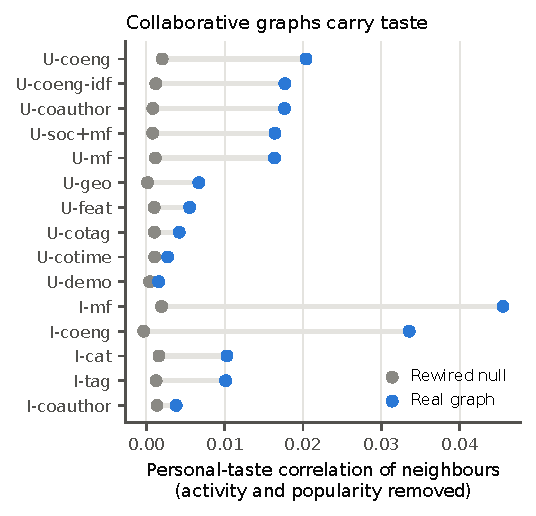
\includegraphics[width=0.48\linewidth]{../figures/fig1_graph_alignment.pdf}\hfill
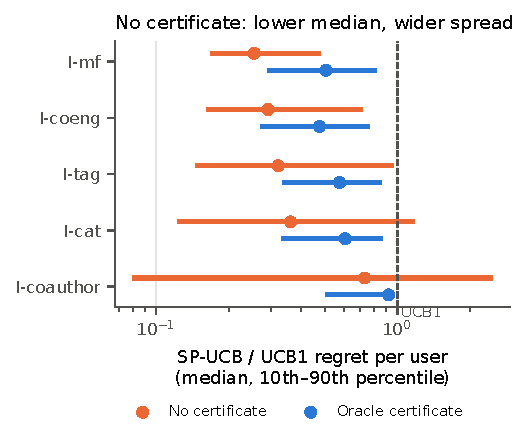
\includegraphics[width=0.48\linewidth]{../figures/fig2_pooling_tails.pdf}
\caption{Left: personal-taste correlation of graph neighbours, real against rewired. Right: SP-UCB regret relative to UCB1 per user (Setting A), without and with an oracle certificate.}\label{fig:align-tails}
\end{figure}

\paragraph{Findings.}
\begin{itemize}
\item Collaborative graphs carry personal taste: I-mf neighbours agree at 0.046 against 0.002 for random pairs; U-coeng is the best user graph (quotient 0.649 against 0.791 for its rewiring). Tag, category and same-author graphs mostly group by popularity; profile, location, demographic and time-of-day graphs are near random.
\item Rankings are stable across $k\in\{5,10,20\}$ and under a binary like-based reward (R3; rank correlation of quotients 0.80).
\item Smoother than chance is not safe to smooth: on most item graphs, fixed smoothing costs more of each user's best-video value than on the rewired null (I-mf at $\lambda=10$: 0.117 against 0.019). Random-graph smoothing behaves like uniform shrinkage, which keeps rankings; real graphs pull items toward their neighbourhood's level, which reorders the top. This is the misalignment mechanism of Section~\ref{sec:mean}, measured.
\item Users' rows correlate at 0.38 even for random pairs, so a shared popularity component dominates user graphs.
\end{itemize}

\subsection{Pooling over items and users}

\paragraph{Setting A (one user, 300 sampled videos, item graph rebuilt on the subset; 60 users, $T=20{,}000$).}
\begin{itemize}
\item Gains come from shrinkage, not structure: on a rewired I-mf graph SpectralUCB at $\lambda=10$ regrets $0.695\times$ UCB1 against $0.697\times$ on the real graph; spectral TS $0.610\times$ against $0.611\times$ graph-free Gaussian TS.
\item Uncertified pooling has heavy tails (Figure~\ref{fig:align-tails}, right). Ratios to Bernoulli TS (median / 90th percentile): spectral TS ($\lambda=10$) on I-mf 0.68 / 1.71, on I-coeng 1.11 / 18.78; SP-UCB without a certificate on I-coauthor 2.06 / 29.61 and on I-cat 1.72 / 11.37; UCB1 4.29 / 14.02.
\item Oracle-certified SP-UCB halves UCB1's regret (I-mf $0.53\times$, I-coeng $0.50\times$) without exceeding UCB1's tail.
\item The energy certificate is too loose: on 300-video instances the energy-to-gap ratio is about 5 for every graph, above the threshold of about 1; energy certificates reject 18--33\% of suboptimal components against 55--83\% for oracle certificates.
\end{itemize}

\begin{table}[t]\centering\small
\begin{tabular}{lcccc}
\toprule
SP-KLUCB certificate (I-mf) & Ratio to KL-UCB (mean / 90th) & Valid & Rejectable & Mean width \\
\midrule
Oracle & 0.78 / 1.05 & 100\% & 63\% & 0.36 \\
Calibrated, 50th percentile & 0.81 / 1.05 & 52\% & 65\% & 0.30 \\
Calibrated, 90th percentile & 1.00 / 1.05 & 93\% & 19\% & 0.71 \\
Energy & 0.98 / 1.05 & 100\% & 18\% & 0.80 \\
None & 0.67 / 1.32 & 0\% & 98\% & 0 \\
\midrule
Per-user calibrated, 90th percentile & 0.96 / 1.05 & 90\% & -- & 0.60 \\
Per-user calibrated, 75th percentile & 0.88 / 1.05 & 73\% & -- & 0.40 \\
\bottomrule
\end{tabular}
\caption{Setting A v2 with KL-based bounds (30 users $\times$ 2 subsets, $T=20{,}000$).}\label{tab:a2}
\end{table}

\paragraph{Setting A v2 (KL bounds, calibrated certificates).} Table~\ref{tab:a2}. Oracle-certified pooling cuts regret 22\% at no tail cost; no practical certificate gets there: energy and 90th-percentile calibrated certificates are valid but too wide; the 50th-percentile calibration is narrow but valid for only half of the components. Uncertified pooling is best on average and worst in the tail, and does as well on the rewired graph.

\paragraph{Per-user calibration.}\label{sec:usercal} Within-component ranges vary too much across users for a population quantile to be both valid and narrow. A per-user certificate first pulls each of the 300 videos once (charged to regret), estimates the user's reward level, and sets each component's width to a quantile of the ranges of the 100 tuning users with the closest level. At the 90th percentile it is valid for 89--90\% of components with mean width 0.55--0.60 (against 0.71 for the population quantile) and regret $0.95$--$0.96\times$ KL-UCB; at the 75th percentile, valid for 73\% with width 0.36--0.40 and regret $0.86$--$0.88\times$ (I-coeng / I-mf). Level matching recovers about half of the oracle's gain, but no practical certificate is yet both valid and narrow.

\paragraph{Setting B (users arrive at random; 300 users $\times$ 100 videos; $T=100{,}000$; 8 instances).} Shrinking each video's estimate toward its population mean (complete graph, $\lambda=10$) cuts regret 27\% against per-user TS; real user graphs do not beat it (U-mf $0.741$, rewired U-coeng $0.745$, U-coeng $0.759$, U-geo $0.893$). Pooling over user clusters with an oracle certificate gains about 6\%; with calibrated certificates nearly nothing; without a certificate regret rises 39\%.

\subsection{Certificates under persistence}\label{sec:exp-cert}

\paragraph{Design.} Twenty arms in four components of five; component bands of width $\varepsilon_c=0.1$; best mean 0.55, others 0.15--0.45; AR(1) fluctuations with $\Var(z)=1$, persistence $\varphi\in\{0,0.5,0.9,0.97\}$, independent or path-graph-correlated shocks; observation noise sd 0.1; $T=5{,}000$; 20--30 seeds. Exposure is one arm at a time ($b=1$) or in blocks of 25 rounds ($b=25$), as in daily slates or batched updates.

\begin{table}[t]\centering\small
\begin{tabular}{lcccc}
\toprule
Exposure & $\varphi$ & Regret: iid / B1 / B1$'$ & iid violated (runs) & B1, B1$'$ violated \\
\midrule
One at a time & 0 & 353 / 753 / \textbf{295} & 0\% & 0\% \\
One at a time & 0.5 & 457 / 752 / \textbf{396} & 0\% & 0\% \\
One at a time & 0.9 & 533 / 759 / 564 & 0\% & 0\% \\
One at a time & 0.97 & 649 / 755 / 679 & 0\% & 0\% \\
Blocks of 25 & 0 & 380 / 766 / \textbf{338} & 0\% & 0\% \\
Blocks of 25 & 0.5 & 406 / 916 / 510 & 5\% & 0\% \\
Blocks of 25 & 0.9 & 629 / 1,023 / 818 & 75\% & 0\% \\
Blocks of 25 & 0.97 & 853 / 1,034 / \textbf{828} & 90\% & 0\% \\
\bottomrule
\end{tabular}
\caption{Certified pooling under persistence, independent shocks (20 seeds).}\label{tab:b1p}
\end{table}

\begin{figure}[t]\centering
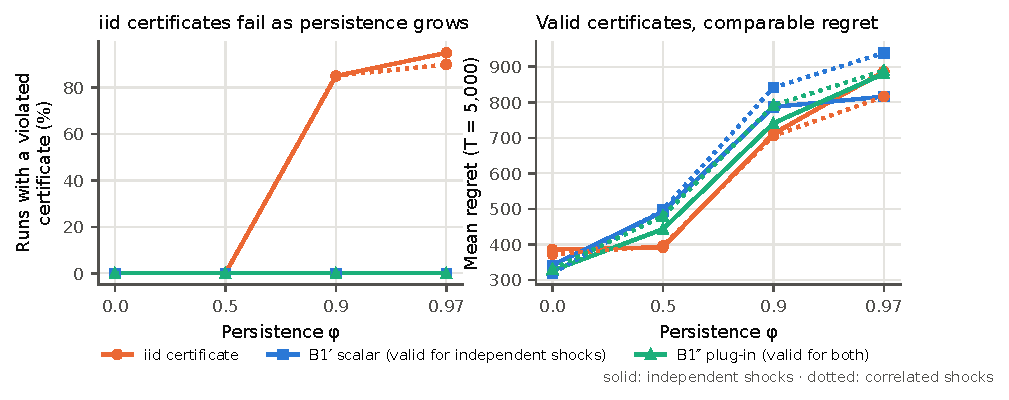
\includegraphics[width=\linewidth]{../figures/fig3_certificates_under_persistence.pdf}
\caption{Bursty exposure (blocks of 25): share of runs with a violated certificate (left) and mean regret (right).}\label{fig:cert}
\end{figure}

\paragraph{Findings.}
\begin{itemize}
\item iid certificates fail under bursty persistent exposure: violated in 70--75\% of runs at $\varphi=0.9$ and 90--100\% at $\varphi=0.97$ (58--88\% of rounds). With one-at-a-time sampling they stay covered, because interleaving decorrelates repeat pulls ($\varphi^{20}\approx0.54$ at $\varphi=0.97$).
\item Innovation-regression certificates are never violated in any configuration.
\item B1 is valid but too wide: it eliminated nothing within 20,000 rounds. B1$'$ removes most of that cost and beats iid pooling when persistence is low (16\% lower regret at $\varphi=0$), is within 6\% at high persistence with one-at-a-time sampling, and is 26--30\% worse at moderate persistence with bursty exposure, where the iid certificate is invalid in up to 75\% of runs.
\item Irrevocable decisions expose the risk: certified successive elimination with iid certificates wrongly eliminated the best arm in 40--75\% of bursty high-persistence runs (at both $T=5{,}000$ and $20{,}000$), against a nominal 5\%; with innovation-regression certificates, never.
\item B1$''$ under correlated shocks (Table~\ref{tab:b1pp}, Figure~\ref{fig:cert}; arm order shuffled, 20 seeds) is never violated. With one-at-a-time sampling it beats iid pooling up to $\varphi=0.9$ (e.g.\ 606 against 642 at $\varphi=0.9$); with bursty exposure it is 9--21\% worse at $\varphi\ge0.5$, exactly where the iid certificate is invalid in 85--90\% of runs. Elimination built on iid certificates wrongly drops the best arm in 35--90\% of bursty high-persistence runs; built on B1$''$, never.
\end{itemize}

\begin{table}[t]\centering\small
\begin{tabular}{lcccc}
\toprule
Exposure & $\varphi$ & Regret: iid / B1$'$ / B1$''$ & iid violated (runs) & B1$''$ violated \\
\midrule
One at a time & 0 & 357 / 317 / \textbf{313} & 0\% & 0\% \\
One at a time & 0.5 & 460 / 383 / 412 & 0\% & 0\% \\
One at a time & 0.9 & 642 / 646 / \textbf{606} & 0\% & 0\% \\
One at a time & 0.97 & 693 / 683 / 760 & 0\% & 0\% \\
Blocks of 25 & 0 & 372 / 319 / 330 & 0\% & 0\% \\
Blocks of 25 & 0.5 & 395 / 497 / 479 & 0\% & 0\% \\
Blocks of 25 & 0.9 & 706 / 841 / 792 & 85\% & 0\% \\
Blocks of 25 & 0.97 & 816 / 939 / 889 & 90\% & 0\% \\
\bottomrule
\end{tabular}
\caption{Correlated shocks (path-graph innovation covariance), shuffled arm order, 20 seeds. B1$'$ has no guarantee here; B1$''$ does.}\label{tab:b1pp}
\end{table}

\subsection{Spatiotemporal benchmark}

\paragraph{Design.} 100 arms on a $10\times10$ grid; AR(20) coefficients proportional to $e^{-r/6}$ summing to 0.97; innovation covariance a unit-diagonal graph resolvent $(I+5L)^{-1}$ (neighbour correlation high); long-run means smooth on the grid, $\mu\sim N(0,0.25\,C)$; observation sd 0.3; $T=2{,}000$; 8 seeds. Configurations: main; weak persistence (sum 0.6); no spatial correlation. Model-based policies know the dynamics and covariance; means are unknown.

\begin{table}[t]\centering\small
\begin{tabular}{llccc}
\toprule
Policy & Uses & Main & No spatial & Weak persistence \\
\midrule
ST UCB, 2 sd & spatiotemporal & \textbf{0.850} (46\%) & \textbf{0.890} & 1.856 \\
ST UCB, 4 sd & spatiotemporal & 0.863 & 0.953 & 1.596 \\
ST predictive sampling & spatiotemporal & \textbf{0.950} (37\%) & 1.057 & 1.568 \\
SpectralUCB & spatial only & 1.026 & 1.014 & 1.953 \\
UCB1 & iid & 1.095 & 1.157 & 1.867 \\
AR predictive sampling & temporal only & 1.121 & 1.094 & \textbf{1.525} \\
ST Thompson sampling (current state) & spatiotemporal & 1.258 & 1.452 & 2.246 \\
Thompson sampling & iid & 1.329 & 1.523 & 1.675 \\
ST two-period score & spatiotemporal & 1.402 & 1.429 & 1.848 \\
ST UCB, theory constant & spatiotemporal & 1.489 & 1.838 & 1.499 \\
ST greedy & spatiotemporal & 1.509 & 1.678 & 1.932 \\
Sliding-window UCB & iid & 1.540 & 1.586 & 2.282 \\
\midrule
Innovation lower bound & & 0.298 & 0.323 & 1.276 \\
\bottomrule
\end{tabular}
\caption{Dynamic regret per round (share of the gap between TS and the lower bound closed, in brackets).}\label{tab:toy}
\end{table}

\begin{figure}[t]\centering
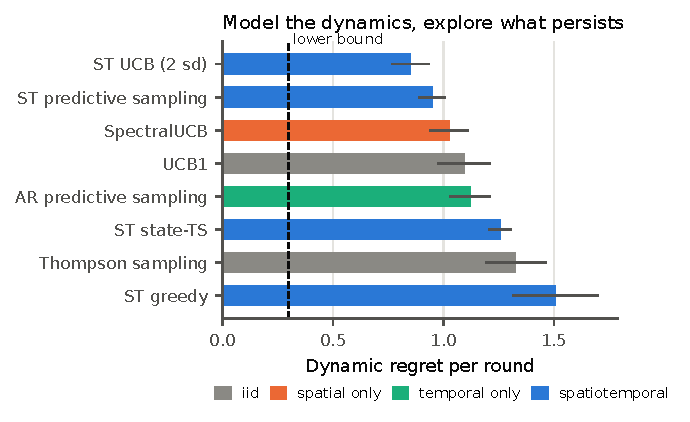
\includegraphics[width=0.48\linewidth]{../figures/fig4_toy_fluctuation_channel.pdf}\hfill
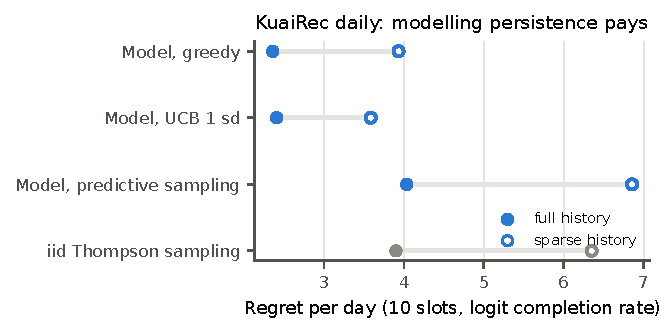
\includegraphics[width=0.48\linewidth]{../figures/fig5_kuairec_daily.pdf}
\caption{Left: spatiotemporal benchmark (main configuration). Right: KuaiRec daily, full against sparse fit-window history.}\label{fig:toy-daily}
\end{figure}

\paragraph{Findings.}
\begin{itemize}
\item The spatiotemporal model wins once exploration targets the right uncertainty. Joint predictive sampling, which has no tuning parameter, cuts dynamic regret 27\% against TS and 13\% against UCB1, closing 37\% of the gap to the lower bound; tuned ST UCB closes 46\% (mild selection bias: multipliers compared on the same runs).
\item Mis-targeted exploration is as harmful as no model: greedy never explores; current-state TS samples the fresh innovation; the theory-constant UCB over-explores. All three lose to UCB1.
\item Spatial correlation adds about 15\% on top of persistence (joint against temporal-only predictive sampling, 0.950 against 1.121).
\item With weak persistence the lower bound is already 1.28 per round and gains shrink.
\end{itemize}

\subsection{KuaiRec daily engagement}

\paragraph{Design.} 253 videos observed on all 63 days; reward the logit daily complete-play rate; ten slots per day; fit windows of $F\in\{28,35,42\}$ days of full logs (AR lags $\{1,2,7\}$; innovation covariance shrunk toward an I-coeng graph kernel plus a common shock); test on the remaining days.

\paragraph{Data.} Deviations persist (lag-1 autocorrelation 0.78; AR spectral radius 0.75--0.81) and are as large as the spread of long-run means (sd 0.46 against 0.54). Shocks are only weakly graph-linked: I-coeng neighbours' innovations correlate at 0.071, against 0.068 on the rewiring and 0.042 for all pairs (a platform-wide common shock).

\begin{table}[t]\centering\small
\begin{tabular}{lcccc}
\toprule
Policy & $F=28$ & $F=35$ & $F=42$ & Mean \\
\midrule
Drift 0.0005 (likelihood-selected), greedy & 2.79 & 3.01 & 1.28 & \textbf{2.36} \\
Spatiotemporal filter, greedy & 3.08 & 2.84 & 1.31 & 2.41 \\
AR filter (temporal only), greedy & 3.15 & 2.80 & 1.35 & 2.44 \\
Persistent sampling (I-coeng / rewired / no graph) & & & & 2.63 / 2.64 / 2.62 \\
ST UCB, 1 sd & 3.04 & 3.11 & 1.57 & 2.57 \\
Last observed value & 4.27 & 3.46 & 0.93 & 2.88 \\
iid Gaussian TS & 3.88 & 4.12 & 3.71 & 3.90 \\
Joint predictive sampling & 3.81 & 4.87 & 3.43 & 4.04 \\
Current-state TS & 4.17 & 5.15 & 4.41 & 4.58 \\
Fit-window means & 4.94 & 5.31 & 4.47 & 4.91 \\
\midrule
\multicolumn{5}{l}{\emph{Sparse history (10 videos seen per fit day)}} \\
ST UCB, 1 sd & 4.23 & 4.23 & 2.30 & \textbf{3.59} \\
ST greedy & 4.35 & 4.03 & 3.42 & 3.93 \\
ST UCB, 2 sd & 5.17 & 6.69 & 3.31 & 5.06 \\
iid TS & 6.34 & 6.65 & 6.06 & 6.35 \\
Joint predictive sampling & 6.14 & 7.53 & 6.89 & 6.85 \\
\bottomrule
\end{tabular}
\caption{KuaiRec daily regret per day (oracle top-10 sum minus chosen sum, logit scale).}\label{tab:daily}
\end{table}

\paragraph{Findings.}
\begin{itemize}
\item Modelling persistence is the consistent real-data win: 38\% (full history) to 43\% (sparse history) less regret than iid TS.
\item The graph adds about 1\% here, matching the weak graph correlation of shocks on KuaiRec.
\item Lifecycle drift: late in the window the stale last-value rule beats every model at $F=42$ (0.93). A small likelihood-selected drift helps overall (2.36); larger drift helps late and hurts early, so drift grows with video age.
\item Exploration value depends on prior information and horizon: with full history greedy is best; with sparse history a 1-sd bonus beats greedy by 9\%; heavier exploration over-explores because the test window offers about one observation per video, against about twenty per arm in the benchmark.
\end{itemize}

\subsection{Wikipedia attention over the hyperlink graph}\label{sec:wiki}

\paragraph{Design.} Arms are the 150 most-viewed English Wikipedia articles linked from ``List of programming languages'' with complete data (512 of 691 had complete series). The panel is daily user page views, 1 January 2022 to 31 December 2025 (1,461 days), from the public Wikimedia REST API. The graph is the 3,037 hyperlinks among them (mean degree 40.5), symmetrized. The reward of featuring an article is $\log(1+\text{views})$; ten articles are featured per day. For origins $F\in\{365,730,1095\}$ the model is fitted on the preceding 365 days (AR lags $\{1,2,7\}$, innovation covariance shrunk toward a hyperlink-graph resolvent plus a common shock) and tested on the next 120 days, with real, rewired and no-graph covariances, a drifting level and a sparse-history variant.

\paragraph{Data.} Attention persists with a weekly cycle (lag-1 autocorrelation 0.72, lag-7 0.74, lag-30 0.37; AR spectral radius 0.97). Shocks are strongly correlated but through a domain-wide factor: innovations correlate at 0.218 across all pairs, 0.256 across hyperlinked pairs and 0.250 across rewired pairs.

\begin{table}[t]\centering\small
\begin{tabular}{lcccc}
\toprule
Policy & $F=365$ & $F=730$ & $F=1095$ & Mean \\
\midrule
Spatiotemporal filter, drifting level, greedy & 0.045 & 0.828 & 0.254 & \textbf{0.376} \\
Joint predictive sampling & 0.085 & 0.848 & 0.287 & 0.407 \\
Spatiotemporal UCB, 1 sd & 0.054 & 0.999 & 0.256 & 0.436 \\
Spatiotemporal greedy (hyperlink / rewired / no graph) & 0.050 & 1.015 & 0.258 & 0.441 / 0.441 / 0.441 \\
AR filter (temporal only), greedy & 0.053 & 1.028 & 0.262 & 0.448 \\
Last observed value & 0.045 & 1.012 & 0.400 & 0.486 \\
Fit-window means & 0.045 & 1.340 & 0.256 & 0.547 \\
iid Thompson sampling & 0.062 & 1.340 & 0.256 & 0.553 \\
\bottomrule
\end{tabular}
\caption{Wikipedia attention: regret per day (top-10 log views).}\label{tab:wiki}
\end{table}

\begin{figure}[t]\centering
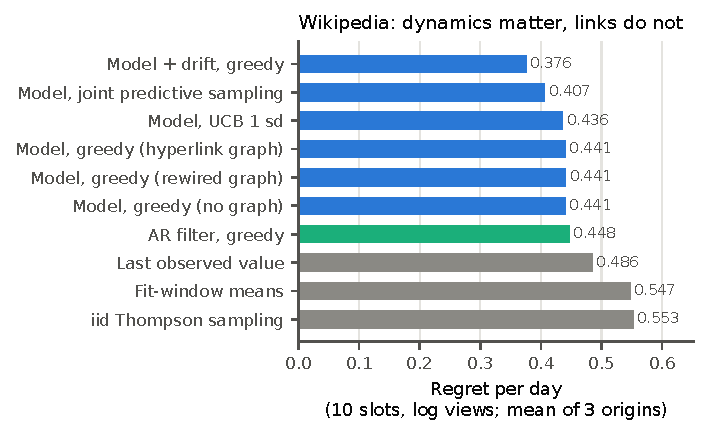
\includegraphics[width=0.55\linewidth]{../figures/fig6_wikipedia.pdf}
\caption{Wikipedia attention over the hyperlink graph, mean regret per day over three origins.}\label{fig:wiki}
\end{figure}

\paragraph{Findings.}
\begin{itemize}
\item Modelling dynamics pays: the drifting-level filter cuts regret 32\% against iid TS and 23\% against the last-value rule.
\item Exploration pays here, unlike on KuaiRec daily: joint predictive sampling is second best ($-26\%$ against TS, 8\% better than greedy without drift). Each article receives about eight observations in the test window, against about one per video on KuaiRec, consistent with matching exploration to observations per arm.
\item Hyperlinks add nothing to the fluctuation model: real, rewired and no-graph covariances tie (0.441). Shocks are shared, but domain-wide rather than along links.
\item Difficulty concentrates where rankings shift (the 2024 window); in stable periods every model is near the oracle.
\end{itemize}

%=====================================================================
\section{Discussion}
%=====================================================================

\paragraph{What the evidence supports.}
\begin{enumerate}
\item Web graphs differ sharply in what they encode. Collaborative and co-engagement graphs carry correlated appeal; social, demographic, location and content-tag graphs carry little beyond popularity.
\item Most pooling gains on KuaiRec come from shrinkage rather than graph structure; rewired graphs match real ones. Structure matters for certification (oracle certificates on real graphs reject more components) and for safety, not for average gains.
\item Uncertified pooling trades a good median for a heavy tail. Certification removes the tail, but practical certificates remain the bottleneck: energy and calibrated certificates are too wide or invalid on real graphs.
\item Persistence must enter confidence sets. Under bursty exposure iid certificates are routinely invalid, and irrevocable decisions built on them fail; innovation-regression certificates are always valid at comparable regret.
\item Modelling dynamics pays on real data (KuaiRec $-38$ to $-43\%$, Wikipedia $-32\%$ against iid TS); exploration must target persistent uncertainty and be matched to the number of observations per arm (it helps on Wikipedia, about eight per arm, and not on KuaiRec daily, about one).
\item Correlated fluctuations on both platforms are dominated by a platform- or domain-wide common shock; neither co-engagement graphs nor hyperlinks carry link-specific shock correlation. Graph-specific fluctuation structure appears in the controlled benchmark (15\% gain) but remains to be found on real web data.
\end{enumerate}

\paragraph{Limitations.} KuaiRec ground truth uses one observed watch ratio per pair, so measured alignment understates preference alignment. Panel experiments assume that showing an item does not change its organic demand. Dynamics are estimated in a fit window and treated as known in the test window. The toy benchmark fixes the model class; real dynamics show lifecycle drift outside it. Regret bounds for B1$'$ and B1$''$ under correlated shocks are stated through realized information; clean per-pull constants exist only for independent AR(1) arms.

\paragraph{Open problems.} (1) A practical, valid, narrow certificate for the mean channel on real graphs. (2) Per-pull information constants under correlated shocks, and the GDE-UCB path rate under persistence. (3) Learning dynamics online with valid certificates. (4) Age-dependent drift for engagement lifecycles.

%=====================================================================
\section{Reproducibility}\label{sec:repro}
%=====================================================================

From the repository root with the virtual environment of \texttt{experiments/kuairec/requirements.txt}:
\begin{verbatim}
python -I experiments/kuairec/data.py
python -I experiments/kuairec/graphs.py --k 5 10 20
python -I experiments/kuairec/alignment.py --k 10
python -I experiments/kuairec/setting_a.py --users 60 --horizon 20000
python -I experiments/kuairec/setting_a2.py --users 30 --subsets 2
python -I experiments/kuairec/setting_b.py --instances 8
python -I experiments/kuairec/daily.py --seeds 5 [--extra | --sparse]
python -I experiments/st_toy/toy.py --seeds 8 [--extra]
python -I experiments/st_toy/coverage.py --tag {_v2,_elim,_scalar,_plugin}
python -I experiments/wikipedia/collect.py
python -I experiments/wikipedia/attention.py [--diagnose]
python -I experiments/paper_figures.py
\end{verbatim}

\end{document}
